\chapter{Implementación del sistema de reconocimiento de gestos propuesto}\label{capit:cap4}
\vspace{-2.0325ex}%
\noindent
\rule{\textwidth}{0.5pt}
\vspace{-5.5ex}% 
\newcommand{\pushline}{\Indp}% Indent puede ir o no :p

En este cap\'itulo se describen los detalles de implementación de cada etapa del sistema.   

\section{Adquisición de los datos}\label{sec:AdquisicionDatos}

Como se vio en el capítulo \ref{capit:cap3} sección \ref{sec:KinectSensor} los datos provienen de los sensores de profundidad de dos dispositivos Kinect, estos se encuentran ubicados uno frente al usuario (Kinect 1), y otro al lado  izquierdo (Kinect 2), con una distancia de $74$ y $79$ $cm.$ respectivamente; y entre ellos de $46$ $cm.$ como se muestra en la figura \ref{fig:SetupSystem}.
\begin{figure}[!h]
\begin{center}
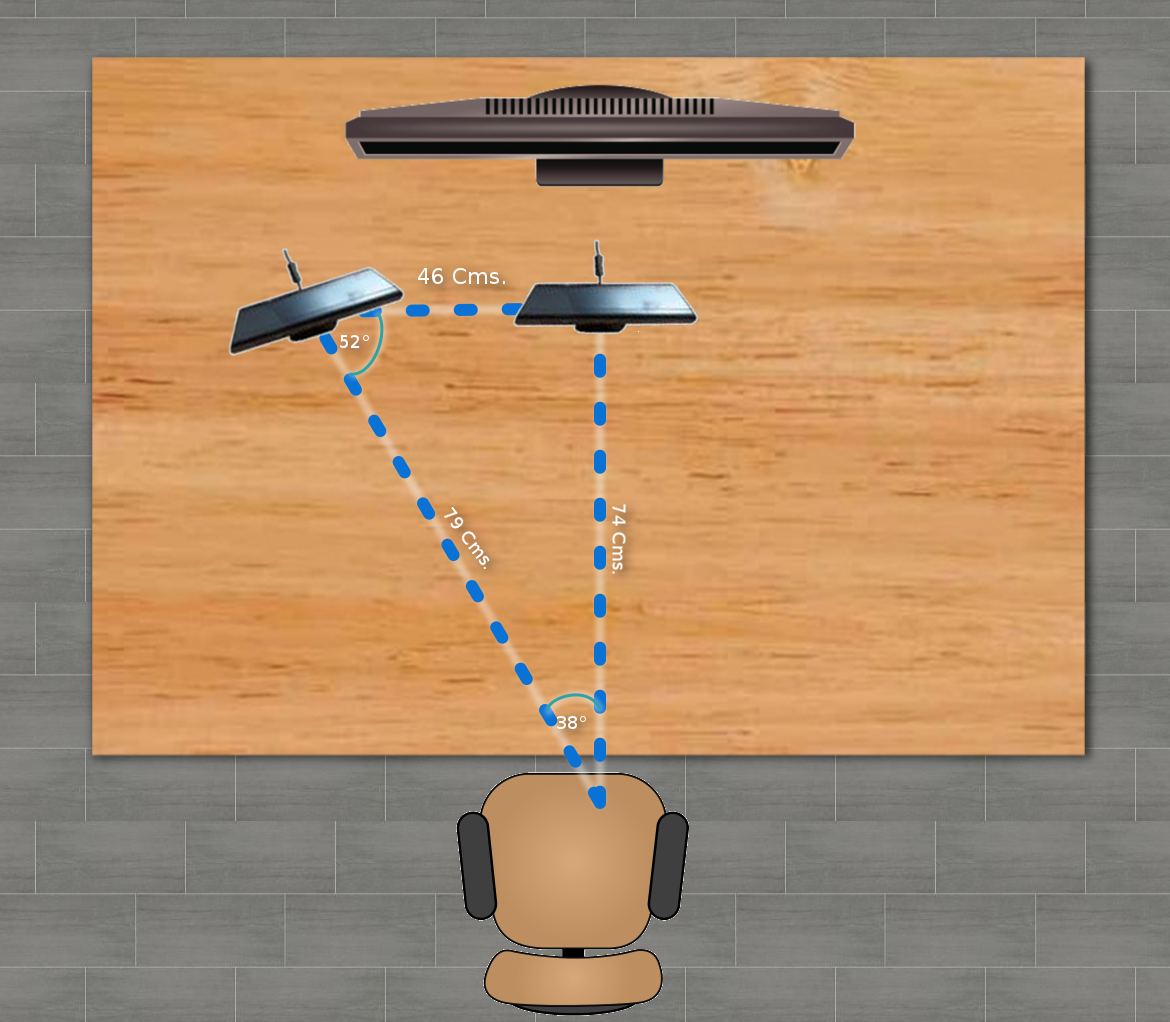
\includegraphics[scale=.2]{./Figures/system.png}
\end{center}
\caption{Configuración del sistema de reconocimiento de gestos}
\label{fig:SetupSystem}
\end{figure}  

Una vez que el flujo de datos de los sensores de profundidad es capturado este es representado como una imagen en escala de grises de $8$ bits de $640$ p\'ixeles de ancho por $480$ p\'ixeles de largo. En las imágenes se puede apreciar detalles pequeños, es decir cambios en la profundidad de hasta $1$  $mm.$ esto debido a que la escala de grises inicia cada $26$  $cm$. 
En la siguiente imagen se puede apreciar un ejemplo de las imágenes de profundidad. \ref{fig:ImagenCapturada}

\begin{figure}[h!]
\begin{center}
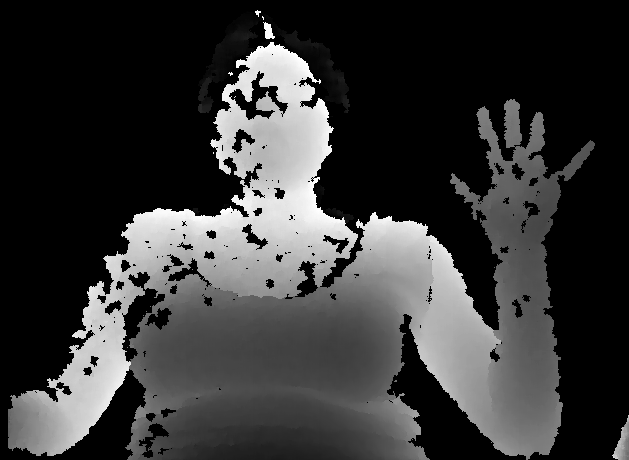
\includegraphics[scale=.5]{./Figures/166.png}
\end{center}
\caption{Representación de los datos capturados por los Kinect}
\label{fig:ImagenCapturada}
\end{figure}  

Por la naturaleza del Kinect, las imágenes obtenidas de ambos sensores contiene ruido, como el se muestra en la figura \ref{fig:ImagenCapturadaNoNoise}; el ruido es reducido usando un filtro de mediana, este es aplicado en toda la imagen usando una ventada de tamaño $13$. La imagen resultante $S(x,y)$ es como la que se muestra en la figura \ref{fig:ImagenCapturadaNoNoise}.\\ 
\begin{figure}[h!]
\begin{center}
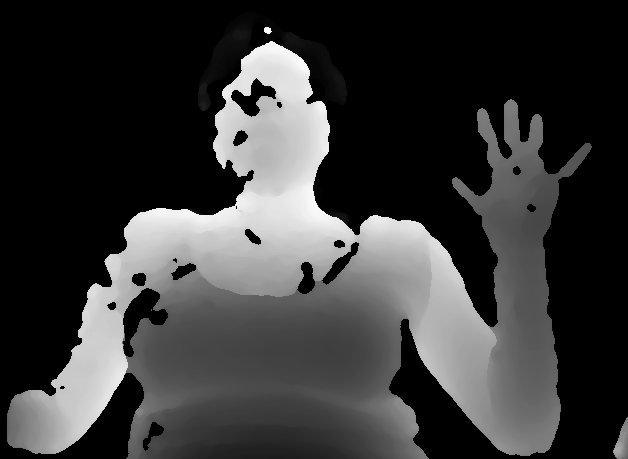
\includegraphics[scale=.5]{./Figures/166_W13.png}
\end{center}
\caption{Representación de los datos capturados por los Kinect}
\label{fig:ImagenCapturadaNoNoise}
\end{figure}  
Se aprecia en la imagen siguiente  que gran parte del ruido es reducido obteniendo una mejora en la imagen, desafortunadamente todavía existe ruido en la imagen, este puede ser eliminado casi en su mayoría  si el tamaño de la ventana aumenta pero se pierde información importante de la imagen, de manera que se decidió optar por el tamaño de ventana, antes mencionado. En la imagen también se aprecia el fondo negro, esto es debido a que se discrimino el fondo que estuviera a un distancia de más de $2$ $m.$ del sensor. 



\section{Detección}\label{sec:DeteccionSystem} 

En este trabajo se utiliza el algoritmo de detección de objetos desarrollado por Viola y Jones (2001), como se mostró en el cap\'itulo \ref{capit:cap3} sección \ref{subsec:ViolaJones}, el algoritmo clasifica las imágenes basándose en el valor de características, el clasificador es construido usando el algoritmo de AdaBoost en forma de cascada. 


La selección de las características se llev\'o acabo por medio de una versión modificada del algoritmo AdaBoost; la implementaci\'on se realiz\'o utilizando el software OpenCV Haar training classifier \footnote{https://github.com/mrnugget/opencv-haar-classifier-training}. Se entren\'o con $1000$ imágenes positivas (imágenes de profundidad de la mano), y $2000$ negativas, (imágenes de fondo de distintos escenarios). Las imágenes positivas fueron generadas de $300$ imágenes de poses; $3$ poses distintas, $100$ de cada pose, usando el software Create Samples \footnote{http://note.sonots.com/SciSoftware/haartraining.html}. Todas las imágenes usadas fueron tomadas de nuestra base de  datos \footnote{\label{myrepo} https://github.com/americamm}.

Nuestra base de datos contiene gran cantidad de imágenes de profundidad. Imágenes de fondo y de poses de la mano, estas fueron tomadas a una distancia de entre $60$ y $200$ $cm$. Las imágenes de profundidad de la mano fueron tomadas de $6$ personas distintas con tres distintas poses: palma con los dedos separados \ref{fig:ImagenesPoses:2}, palma con dedos juntos \ref{fig:ImagenesPoses:3} y finalmente el pu\~no \ref{fig:ImagenesPoses:1}, como se muestran en la figura \ref{fig:ImagenesPoses}. Las imágenes de fondo fueron tomadas de distintos escenarios como se muestra en la figura \ref{fig:ImagenFondo}. El programa de captura de las imágenes puede ser encontrado en Github \ref{myrepo}.  

\begin{figure}[h!]
\begin{center}
\subfigure[Palma de la mano con los dedos separados.]{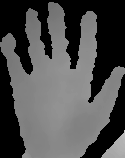
\includegraphics[scale=1]{./Figures/TrainingImage2.png}\label{fig:ImagenesPoses:2}}      \quad
\subfigure[Puño.]{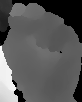
\includegraphics[scale=1.55]{./Figures/TrainingImage1.png}\label{fig:ImagenesPoses:1}}   \quad
\subfigure[Palma de la mano con los dedos juntos.]{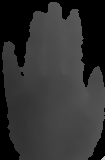
\includegraphics[scale=.99]{./Figures/TrainingImage3.png}\label{fig:ImagenesPoses:3}}
\end{center}
\caption{Ejemplo de imágenes de poses de nuestra base de datos.}
\label{fig:ImagenesPoses}
\end{figure}  

\begin{figure}[h!]
\begin{center}
\subfigure[Ejemplo de imagen de fondo, donde se encuentra una silla y escritorio]{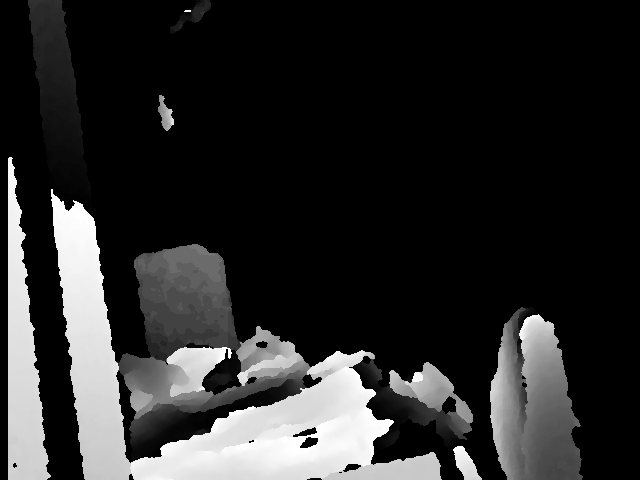
\includegraphics[scale=.3]{./Figures/Fondo5262.png}}\quad 
\subfigure[Ejemplo de imagen de fondo, ]{
\includegraphics[scale=.3]{./Figures/pusheen.png}}\quad 
\end{center}
\caption{Imágenes del fondo de nuestra base de datos.}
\label{fig:ImagenFondo}
\end{figure}  

Los parámetros utilizados para la obtención del clasificador final fueron: el porcentaje de precision de detección de [$\%$] y la tasa de falsos positivos aceptados de [$\%$]. El resultado final del entrenamiento fue en clasificador AdoBoost en forma de cascada, que consta de 19 etapas. El clasificador resultante se encuentra en Github \ref{myrepo}, en formato XML.  

Con el clasificado obtenido, se localiza la mano en cada cuadro proveniente de los dispositivos  Kinect, una ventana  inicial de tamaño $ka$ se desliza por la imagen. Para eliminar falsos positivos que pudieran ocurrir en la detección de la mano se utiliza un algoritmo equivalente al de [referencia], este se muestra en el apéndice \ref{chap:apendA}.\\ 
Una vez que la mano se localiza la región de interés $ROI(x,y)$ es seleccionada alrededor de la mano, como se observa en la figura \ref{fig:Roi}.

\begin{figure}[h!]
\begin{center}
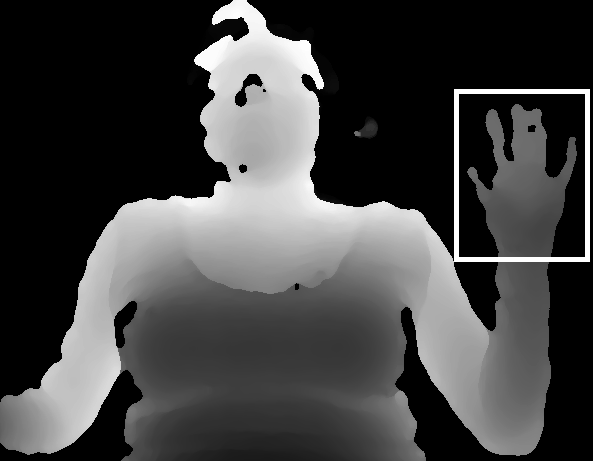
\includegraphics[scale=.5]{./Figures/roi.png}
\end{center}
\caption{Localización y selección de la mano, en la imagen de entrada del Kinect 1.}
\label{fig:Roi}
\end{figure}  

Ya que se tiene localizada el área donde se encuentra la mano, el siguiente paso es segmentar la mano del ROI. La segmentación se realiza binarizando el área del ROI, solo se toma esta área, para que el proceso sea más rápido. La binarizacion se lleva acabo usando el algoritmo de Otsu, el resultado se muestra en la figura \ref{fig:BinarizationRoi}. 
  
\begin{figure}[h!]
\begin{center}

\includegraphics[scale=.5]{./Figures/pusheen.png}
\end{center}
\caption{Binarización de ROI}
\label{fig:BinarizationRoi}
\end{figure} 

En la imagen [agregar imagen feita binarizada], se observa que el resultado de la bianrizacion no es el esperado. Para mejorar la binarizacion, el ruido existe en la imagen es eliminado aplicando dos operaciones morfológicas, apertura y cierre, en ese orden.\\
Las operaciones anteriores utilizan un elemento estructural rectangular; para la operación de apertura el tamaño del elemento es de $3 \, x \, 9$ pixeles; para el cierre se aplic\'o con un tamaño  $3\, x \, 11$ pixeles.
Las imágenes siguientes muestran el resultado de aplicar las operaciones apertura y cierre al ROI.  

\begin{figure}[h!]
\begin{center} 
\subfigure[]{
\includegraphics[scale=0.4]{./Figures/pusheen.png}\label{fig:HandNoNoises:1}}   \qquad
\subfigure[]{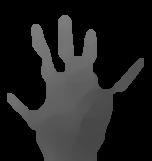
\includegraphics[scale=1.1]{./Figures/65_C.png}\label{fig:HandNoNoises:2}}  
\end{center}
\caption{La imágenes muestran el resultado de aplicar las operaciones morfológicas de apertura y cierre.}
\label{fig:HandNoNoises}
\end{figure}  


\section{Extracción de características}\label{sec:ExtraccionCaracteristicasSystem}

Como se vio en el capítulo \ref{capit:cap3} sección \ref{sec:Convexhull} las características de la mano son extraídas utilizando los algoritmos de envolvente convexa y  defectos de convexidad.\\
La figura muestra un ejemplo de la aplicación de estos algoritmos al ROI binarizado.  

\begin{figure}[!h]
\begin{center}

\includegraphics[scale=.5]{./Figures/pusheen.png}
\end{center}
\caption{En esta dibujado la envolvente convexa, los puntos dibujados son los defectos de convexidad, en azul se encuentran los puntos de profundidad y en rojo los puntos de inicio.}
\label{fig:Convex&Defects}
\end{figure}


Una vez aplicados estos dos algoritmos se calcula: el número de dedos levantados, la posición de la punta de los dedos, \ref{fig:FeaturesOfHand} , la posición de la raíz de los dedos, \ref{fig:FeaturesOfHand} , el centro de la palma de mano, \ref{fig:FeaturesOfHand} , los ángulos que existe del centro de la mano a la punta de los dedos, los ángulos que existen del centro a la raíz de los dedos, la distancia que existe del centro de los dedos a la raíz de los dedos. y las puntas de estos que son fundamentales para calcular las demás características. En la imagen siguiente se muestran algunas de estas características.  

\begin{figure}[h!]
\begin{center} 

\includegraphics[scale=0.6]{./Figures/pusheen.png}
\end{center}
\caption{Resultado del cálculo de las características de la mano.Se muestra en color azul la punta de los dedos, en color verde la posición de la raíz de los dedos y en rojo el centro de la palma de la mano.}
\label{fig:FeaturesOfHand}
\end{figure}

Para la implementación de las características, se tomo parte del código proveniente de \footnote{buscar la pagina ;/}. 

Las características se guardan en un vector de características de dimensión $ dimension$. La valor de la dimension del vector esta dada por la unión del conjunto de características obtenidas por cada imagen de la mano  obtenida por cada Kinect. En cada vector las características provenientes del Kinect 1 son almacenadas primero seguidas de las del Kinect 2.



\section{Reconocimiento}\label{sec:ReconocimientoSystem}

En este trabajo se reconocen gestos estáticos y dinámicos utilizando el algoritmo de clasificación de máquina de soporte vectorial.  

Como se vio en el capitulo \ref{capit:cap3} sección \ref{sec:SVM} SVM es un algoritmo de aprendizaje de máquina supervisado, por lo que es necesario tener imágenes de los gestos a reconocer ya que con estas el clasificador es entrenado y el modelo de clasificación puede ser creado. 

La implementación de SVM se lleva acabo usando LibSVMSharp \footnote{https://github.com/ccerhan/LibSVMsharp} un wrapper de la librería LibSVM \citep{Chang2011}.

\subsection{Reconocimiento de gestos estáticos}\label{RecognitionEstatic}

El sistema reconoce dos gestos estáticos: el puño y la palma de la mano con los dedos separados.  Para el entrenamiento se tomaron $num$ imágenes de los dos distintos gestos como los de la fig \ref{fig:SVMTrainingStatic}, divididas en partes iguales. De tamaño $640$ por $480$ pixeles.   

\begin{figure}[h!]
\begin{center}
\subfigure[Palma de la mano con los dedos separados.]{
\includegraphics[scale=.5]{./Figures/pusheen.png}\label{fig:SVMTrainingStatic:1}}      \quad
\subfigure[Puño.]{
\includegraphics[scale=.5]{./Figures/pusheen.png}\label{fig:SVMTrainingStatic:2}}
\end{center}
\caption{Ejemplo de imágenes de poses de nuestra base de datos.}
\label{fig:SVMTrainingStatic}
\end{figure}

Para el entrenamiento de la máquina de soporte se utilizo un kernel exponencial, (poner los demás parámetros) y se utilizó validación cruzada con 5 pliegues. 

\subsection{Reconocimiento de gestos dinámicos}\label{RecognitionDynamic}

El sistema reconoce numero de gestos dinámicos.  

%\subsection{Extracción de parámetros}
%Ecuación \ref{eq:gravedad}. 
%
%\begin{equation} \label{eq:gravedad}
%A_{d} = -g - \frac{\sum F}{mass}
%\end{equation} 

%Donde $A_{d}$ representan la aceleración que se aplica a un dispositivo, $g$ la constante de gravedad de 9.81 m/$s^{2}$, y $\sum F$ las fuerzas que se aplican al propia sensor.

%Text  \ref{eq:demandaOxigeno_personalizada} and more $O_{2}$ text:
%
%\begin{equation} \label{eq:demandaOxigeno_personalizada}
%\begin{split} 
%& K = R + H + V \\ 
%& R = 3.5 - (0.0367 \times BMI) - (0.0038 \times age) + (0.1790 \times gender)\\
%& H = 0.1 \times \textrm{velocidad de desplazamiento}\\ 
%& V = 1.8 \times \textrm{velocidad de desplazamiento}\\ 
%\end{split} 
%\end{equation} 
%
%Donde $1 + 2$ representan el consumo de $O_{2}$ en reposo personalizado al usuario $(ml \times kg^{-1} \times min^{-1})$ \citep{Barstow:1991}, $H$ el componente horizontal relativo a la velocidad de desplazamiento (m/min), $V$ el componente vertical relativo a la velocidad (m/min) y pendiente de desplazamiento (\%).
%
%\begin{description}
%  \item[Velocidad:] \hfill \\
%  	Para obtener la velocidad de desplazamiento se utiliza el número de pasos realizados por el usuario como se muestra a continuación (Ecuación \ref{eq:velocidad}).
%  
%\begin{equation} \label{eq:velocidad}
%  S_{k} = D_{k}/W \hspace{10 mm} 
%  D_{k} = ST_{k} \times SL \hspace{10 mm}
%  SL = D_{total}/ST_{total} 
%\end{equation}
%\end{description}
	
\newpage
%%=====================================================

